\begin{appendix}

\chapter{Patrons implémentés pour décrire un carrefour}
\label{annexe:patrons}

\section*{Patron de la description générale}

\begin{minted}[linenos, frame=lines, fontsize=\small]{python}
def description(f):
  phrase = S("Le carrefour à l'intersection")
  # Boucle qui compose la conjonction
  # Permet d'obtenir un texte type "de a, de b et de c"
  et = CP(C("et"))
  for nom in f["noms_branches"]:
    et.add(
      # Le syntagme prépositionnel permet d'obtenir la préposition
      # correspondant au type de voie: "de l'avenue", "du cours", etc.
      PP(
        P("de"),
        D("le"),
        N(nom["type"]),
        nom["name"]
      )
    )
  phrase.add(et)
  phrase.add("est un carrefour à %s branches"%f["nombre_branches"])
  return(json.dumps(phrase.toJSON()))
\end{minted}

\section*{Patron de la description des branches}

\begin{minted}[linenos, frame=lines, fontsize=\small]{python}
def description(f):
  voies = json.loads(f["voies"])
  # Composition de la première partie de la phrase: 
  # "La branche numéro 2 qui s'appelle avenue Roosevelt est composée"
  phrase = S("La branche numéro",  NO(f["numero_branche"]).nat(True), 
             "qui s'appelle", f["nom"]["type"], f["nom"]["name"], 
             "est composée")
    
  # Boucle qui compose la conjonction
  et_global = CP(C("et"))
  for group in voies:
    direction = group["direction"]
    lanes = group["lanes"]
    et_lanes = CP(C("et"))
    for lane in lanes:
      # Pour chaque voie, on ajoute le texte "n voie(s) de type"
      et_lanes.add(NP( 
        P("de"), NO(lane["number"]).nat(True), N("voie"), 
        P("de"), N(lane["type"]) 
      ))
    # On ajoute le texte "entrante(s) ou sortante(s)"
    et_global.add(S(NP (et_lanes, A(direction))))
  phrase.add(et_global)
  return(json.dumps(phrase.toJSON()))
\end{minted}

\section*{Patron de la description des traversées}

\begin{minted}[linenos, frame=lines, fontsize=\small]{python}
def description(f):
    texte = []
    # Première phrase. Indication du nombre de passages piétons de la traversée
    phrase = S("La branche numéro",  NO(f["numero_branche"]).nat(True), 
               "se traverse en", NP(NO(f["nombre_passage_pieton"]).nat(True), 
               N("fois")))
    texte.append(phrase.toJSON())
    # Deuxième phrase. Indication de la présence d'un feu piéton.
    phrase = S("Les passages piéton")
    if f["feux_pieton"] == "complet" : 
        phrase.add("sont tous protégés par un feu")
    elif f["feux_pieton"] == "incomplet" : 
        phrase.add("ne sont pas tous protégés par un feu")
    else : phrase.add("ne sont pas protégés par des feux")
    texte.append(phrase.toJSON())
    # Troisième phrase. Indication de la présence de BEV.
    phrase = S("Ils")
    if f["pavage_tactile"] == "complet" : 
        phrase.add("ont tous des bandes d'éveil de vigilance")
    elif f["pavage_tactile"] == "incomplet" : 
        phrase.add("n'ont pas tous des bandes d'éveil de vigilance")
    else : phrase.add("n'ont pas de bandes d'éveil de vigilance")
    texte.append(phrase.toJSON())
    return(json.dumps(texte))
\end{minted}

\chapter{Exemples de descriptions générées}
\label{annexe:exemples}

Cette annexe présente quatre exemples de descriptions de carrefour générées par la chaîne présentée en chapitre \ref{chap:implementation}. Les données \gls{osm} ont été traitées par crseg pour segmenter le carrefour, puis par crmodel pour générer les informations piétonnes. Enfin, les patrons de descriptions détaillés en annexe \ref{annexe:patrons} ont été appliqués pour générer les descriptions. Les figures présentées contiennent les branches et cœurs de carrefour produits par crseg. Les traversées, îlots et trottoirs ont été produits par crmodel. Les îlots et trottoirs sont présentés dans les figures de manière graphique pour illustrer leur présence, mais ne sont contenus que sous forme d'attribut dans les tronçons qu'ils longent.

\newpage
\section*{Exemple 1}

Sur ce carrefour en croix, le résultat correspond à la réalité du terrain.

\begin{figure*}[ht]
  \centering
  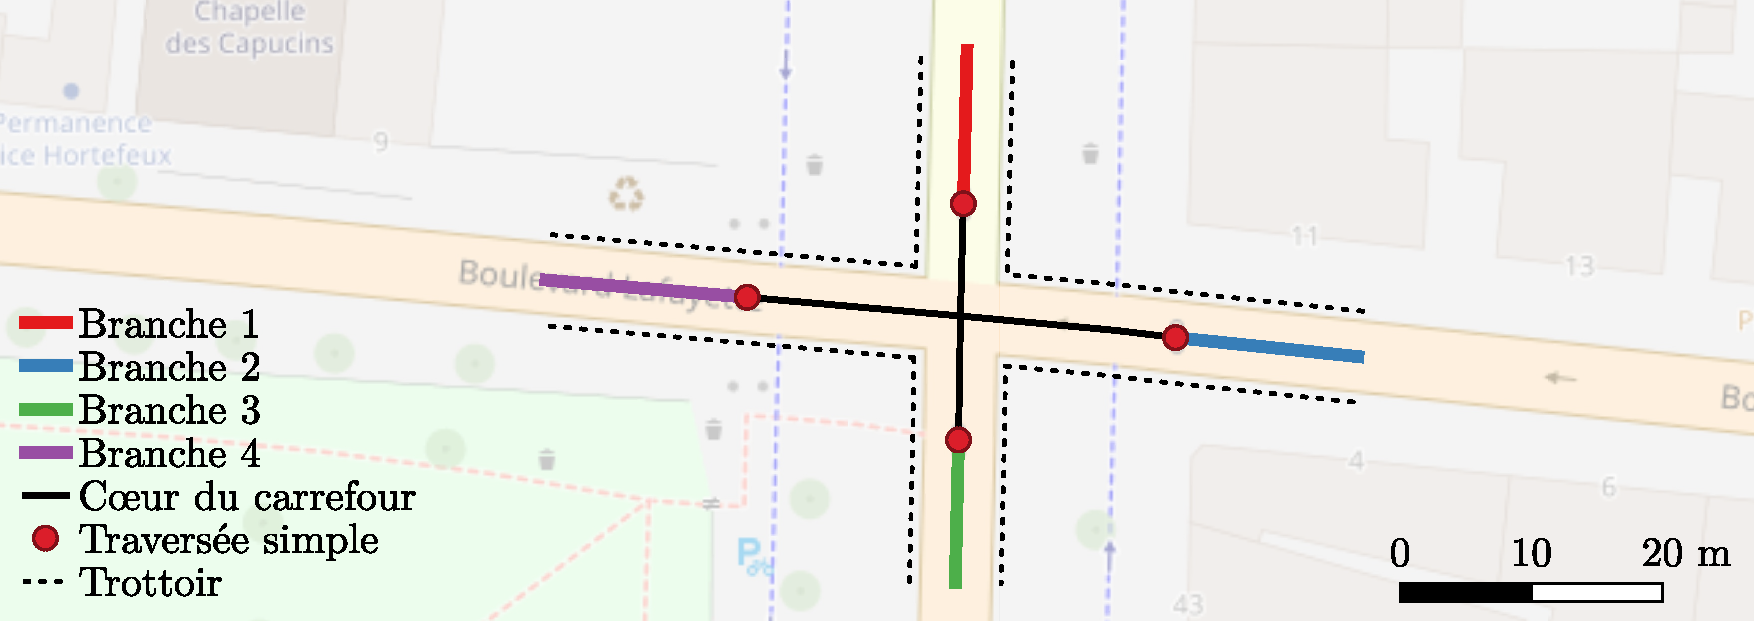
\includegraphics[width=\textwidth]{images/annexes/carrefour_simple.pdf}
  \label{fig:exemple1}
\end{figure*}

Le carrefour à l'intersection du cours Sablon et du boulevard Lafayette est un carrefour à 4 branches.

\newpar{}

La branche numéro un qui s'appelle cours Sablon est composée de deux voies de circulation sortantes, et deux voies de circulation entrantes.

La branche numéro deux qui s'appelle boulevard Lafayette est composée de deux voies de circulation sortantes.

La branche numéro trois qui s'appelle cours Sablon est composée de deux voies de circulation sortantes, et deux voies de circulation entrantes.

La branche numéro quatre qui s'appelle boulevard Lafayette est composée de deux voies de circulation entrantes.

\newpar{}

La branche numéro un se traverse en une fois. Les passages piétons sont tous protégés par un feu. Il y a des bandes d'éveil de vigilance.

La branche numéro deux se traverse en une fois. Les passages piétons sont tous protégés par un feu. Il y a des bandes d'éveil de vigilance.

La branche numéro trois se traverse en une fois. Les passages piétons sont tous protégés par un feu. Il y a des bandes d'éveil de vigilance.

La branche numéro quatre se traverse en une fois. Les passages piétons sont tous protégés par un feu. Il y a des bandes d'éveil de vigilance.

\newpage
\section*{Exemple 2}

La contre-allée au nord-ouest du carrefour n'est pas décrite. Le problème provient de la segmentation, qui ne gère pas les parties déconnectées du reste du carrefour.

\begin{figure*}[ht]
  \centering
  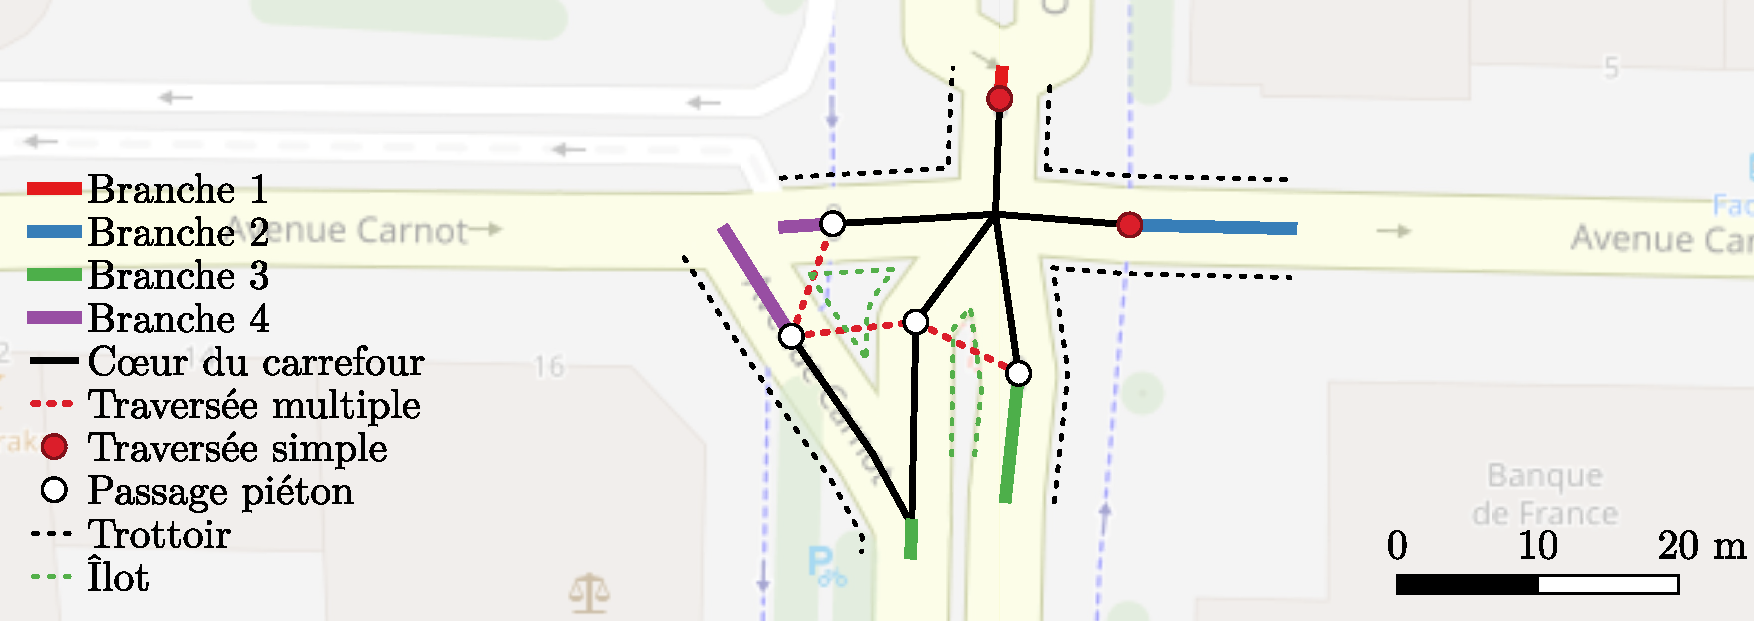
\includegraphics[width=\textwidth]{images/annexes/carrefour_master.pdf}
  \label{fig:exemple2}
\end{figure*}

Le carrefour à l'intersection du cours Sablon et de l'avenue Carnot est un carrefour à 4 branches.

\newpar{}

La branche numéro un qui s'appelle cours Sablon est composée d'une voie de circulation sortante, et trois voies de circulation entrantes.

La branche numéro deux qui s'appelle avenue Carnot est composée d'une voie de bus sortante, et une voie de circulation et une voie de bus entrante.

La branche numéro trois qui s'appelle cours Sablon est composée d'une voie de circulation sortante, et deux voies de circulation entrantes.

La branche numéro quatre qui s'appelle avenue Carnot est composée de quatre voies de circulation sortantes.

\newpar{}

La branche numéro un se traverse en une fois. Les passages piétons sont tous protégés par un feu. Il y a des bandes d'éveil de vigilance.

La branche numéro deux se traverse en une fois. Les passages piétons sont tous protégés par un feu. Il y a des bandes d'éveil de vigilance.

La branche numéro trois se traverse en trois fois. Les passages piétons ne sont pas tous protégés par un feu. Il manque des bandes d'éveil de vigilance ou celles-ci sont dégradées.

La branche numéro quatre se traverse en deux fois. Les passages piétons ne sont pas tous protégés par un feu. Il manque des bandes d'éveil de vigilance ou celles-ci sont dégradées.

\newpage
\section*{Exemple 3}

La traversée simultanée des branches 2 et 3 n'est pas décrite sur ce carrefour. Le problème provient de crmodel qui ne gère les traversées que sur une seule branche à la fois.

\begin{figure*}[ht]
    \centering
    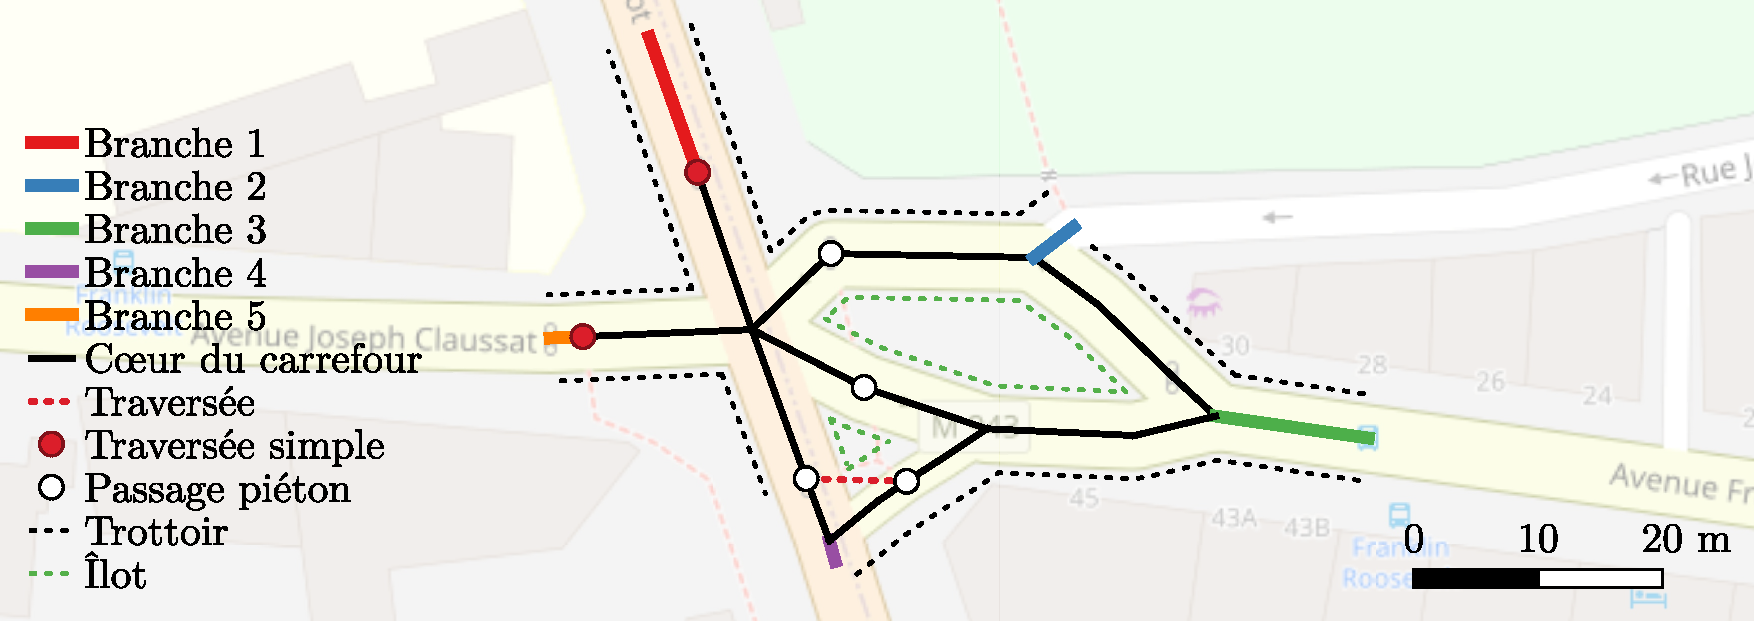
\includegraphics[width=\textwidth]{images/annexes/carrefour_manon.pdf}
    \label{fig:exemple3}
\end{figure*}

Le carrefour à l'intersection du boulevard Berthelot, de la rue Jean-Baptiste Torrilhon, de l'avenue Franklin Roosevelt et de l'avenue Joseph Claussat est un carrefour à 5 branches.

\newpar{}

La branche numéro un qui s'appelle boulevard Berthelot est composée d'une voie de circulation sortante, et deux voies de circulation entrantes.

La branche numéro deux qui s'appelle rue Jean-Baptiste Torrilhon est composée d'une voie de circulation sortante.

La branche numéro trois qui s'appelle avenue Franklin Roosevelt est composée d'une voie de circulation entrante.

La branche numéro quatre qui s'appelle boulevard Berthelot est composée de deux voies de circulation sortantes, et une voie de circulation entrante.

La branche numéro cinq qui s'appelle avenue Joseph Claussat est composée d'une voie de circulation sortante, et deux voies de circulation entrantes.

\newpar{}

La branche numéro un se traverse en une fois. Les passages piétons sont tous protégés par un feu. Il n'y a pas de bandes d'éveil de vigilance.

La branche numéro deux ne se traverse pas.

La branche numéro trois ne se traverse pas.

La branche numéro quatre se traverse en deux fois. Les passages piétons sont tous protégés par un feu. Il manque des bandes d'éveil de vigilance ou celles-ci sont dégradées.

La branche numéro cinq se traverse en une fois. Les passages piétons sont tous protégés par un feu. Il y a des bandes d'éveil de vigilance.

\newpage
\section*{Exemple 4}

La traversée présentée pour la branche 3 est sélectionnée par crmodel car plus courte que les autres solutions. Elle paraît cependant très éloignée du cœur du carrefour et ne serait pas forcément à privilégier.

\begin{figure*}[ht]
    \centering
    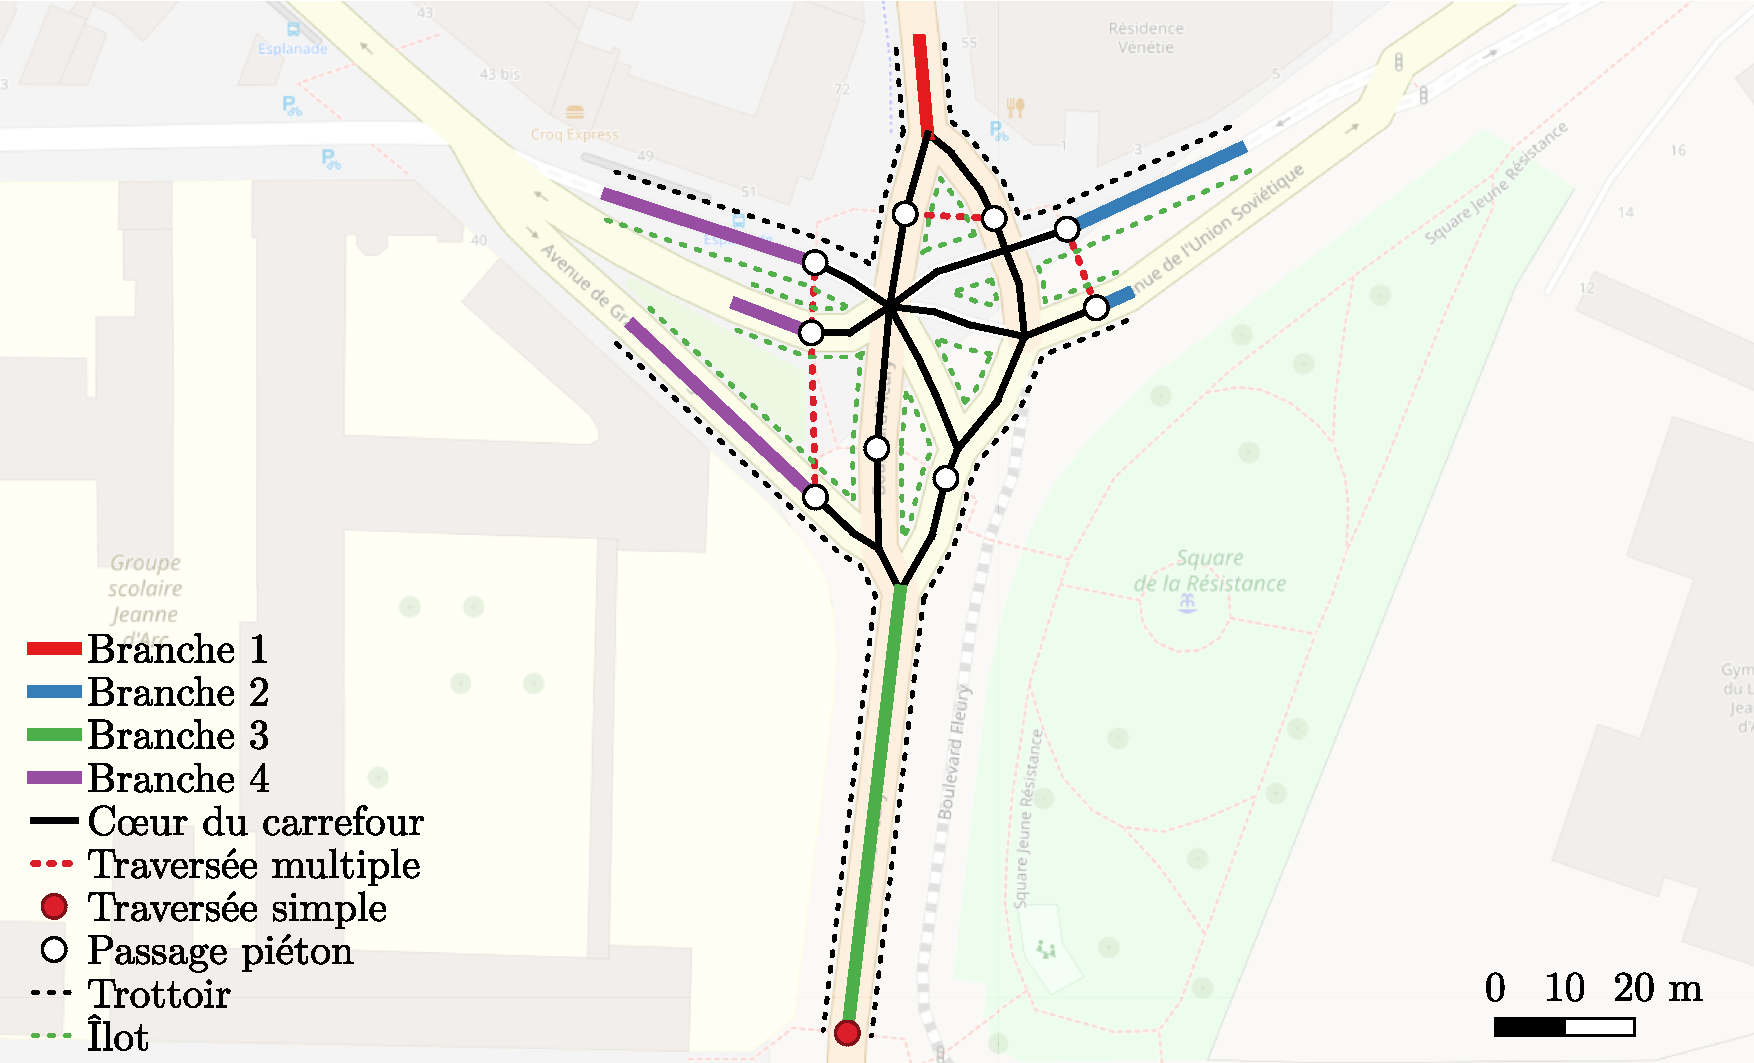
\includegraphics[width=\textwidth]{images/annexes/carrefour_gauthier.pdf}
    \label{fig:exemple4}
\end{figure*}

Le carrefour à l'intersection de l'avenue d'Italie, de l'avenue de l'Union Soviétique, du boulevard Fleury et de l'avenue de Grande-Bretagne est un carrefour à 4 branches.

\newpar{}

La branche numéro un qui s'appelle avenue d'Italie est composée de deux voies de circulation entrantes.

La branche numéro deux qui s'appelle avenue de l'Union Soviétique est composée d'une voie de bus sortante, et deux voies de circulation entrantes.

La branche numéro trois qui s'appelle boulevard Fleury est composée de deux voies de circulation sortantes, et deux voies de circulation entrantes.

La branche numéro quatre qui s'appelle avenue de Grande-Bretagne est composée d'une voie de circulation et une voie de bus sortante, et une voie de circulation et une voie de bus entrante.

\newpar{}

La branche numéro un se traverse en deux fois. Les passages piétons sont tous protégés par un feu. Il y a des bandes d'éveil de vigilance.

La branche numéro deux se traverse en deux fois. Les passages piétons sont tous protégés par un feu. Il manque des bandes d'éveil de vigilance ou celles-ci sont dégradées.

La branche numéro trois se traverse en une fois. Les passages piétons sont tous protégés par un feu. Il y a des bandes d'éveil de vigilance.

La branche numéro quatre se traverse en trois fois. Les passages piétons ne sont pas tous protégés par un feu. Il y a des bandes d'éveil de vigilance.

\chapter{Réponses au questionnaire envoyé aux \glsentryname{ia}s}
\label{annexe:questionnaire}


\section*{Légende}

\newcommand{\qreform}[1]{\hlc[yellow]{#1}}
\newcommand{\qreformcplx}[1]{\hlc[orange]{#1}}
\newcommand{\qsansaj}[1]{\hlc[green]{#1}}
\newcommand{\qavecaj}[1]{\hlc[cyan]{#1}}
\newcommand{\qcorrec}[1]{\hlc[red]{#1}}
\newcommand{\qcomment}[1]{\hlc[pink]{#1}}

\qreform{Reformulation simple}

\qreformcplx{Reformulation complexe}

\qsansaj{Nouvelle informations sans ajout de données}

\qavecaj{Nouvelle informations avec ajout de données}

\qcorrec{Correction de l'information sans reformulation}

\qcomment{Commentaire}

\section*{ID 39}

\label{annexe:q_ID39}

\subsection*{Carrefour 1}

\label{annexe:q_ID39_carrefour1}

Le carrefour à l'intersection du cours Sablon et de l'avenue Carnot est un carrefour à 4 branches.

\newpar{}

La branche numéro un qui s'appelle cours Sablon est composée \qavecaj{d'une contre-allée sortante}, de trois voies de circulation sortantes, et deux voies de circulation entrantes.

\newpar{}

La branche numéro deux qui s'appelle avenue Carnot est composée d'une voie de bus sortante, et une voie de circulation et une voie de bus entrante.

\newpar{}

La branche numéro trois qui s'appelle cours Sablon est composée de deux voies de circulation sortantes, \qcorrec{et trois voies de circulation entrantes}, \qsansaj{dont l'une arrivant directement de la branche numéro quatre, sans passer par le coeur du carrefour}.

\newpar{}

La branche numéro quatre qui s'appelle avenue Carnot est composée de trois voies de circulation sortantes, \qsansaj{dont l'une partant directement vers la branche numéro quatre, sans passer par le coeur du carrefour}, et une voie de bus entrante.

\newpar{}

La branche numéro un se traverse en deux fois. Les passages piétons sont tous protégés par un feu. Il y a des bandes d'éveil de vigilance, \qavecaj{sauf au niveau}\footnote{On suppose sur cette réponse que la phrase est incomplète.}.

\newpar{}

La branche numéro deux se traverse en une fois. Les passages piétons sont tous protégés par un feu. Il y a des bandes d'éveil de vigilance.

\newpar{}

La branche numéro trois se traverse en trois fois. Les passages piétons ne sont pas tous protégés par un feu. Il manque des bandes d'éveil de vigilance ou celles-ci sont dégradées.

\newpar{}

La branche numéro quatre se traverse en trois fois. Les passages piétons ne sont pas tous protégés par un feu. Il manque des bandes d'éveil de vigilance ou celles-ci sont dégradées.

\subsection*{Carrefour 2}

\label{annexe:q_ID39_carrefour2}

Le carrefour à l'intersection du boulevard Berthelot, de la rue Jean-Baptiste Torrilhon, de l'avenue Franklin Roosevelt et de l'avenue Joseph Claussat est un carrefour à 5 branches.

\newpar{}

La branche numéro un qui s'appelle boulevard Berthelot est composée de deux voies de circulation sortantes, et d'une voie de circulation entrante.

\newpar{}

La branche numéro deux qui s'appelle rue Jean-Baptiste Torrilhon est composée de \qcorrec{trois voies de circulation sortantes}.

\newpar{}

La branche numéro trois qui s'appelle avenue Franklin Roosevelt est composée de \qsansaj{deux voies de circulation entrantes, dont l'une arrivant directement de la branche numéro quatre}.

\newpar{}

La branche numéro quatre qui s'appelle boulevard Berthelot est composée de \qsansaj{trois voies de circulation sortantes,  dont l'une partant directement vers la branche numéro trois}, et une voie de circulation entrante.

\newpar{}

La branche numéro cinq qui s'appelle avenue Joseph Claussat est composée \qcorrec{de deux voies de circulation sortantes, et d'une voie de circulation entrante}.

\newpar{}

La branche numéro un se traverse en une fois. Le passage piéton est protégé par un feu. Il n'y a pas de bandes d'éveil de vigilance.

\newpar{}

\qsansaj{Les branches numéro deux et trois se rejoignent en partie en amont du carrefour et se traversent ensemble}. \qreform{La traversée se fait en trois fois}. Les passages piétons sont tous protégés par des feux. Il manque des bandes d'éveil de vigilance ou celles-ci sont dégradées.

\newpar{}

La branche numéro quatre se traverse en deux fois. Les passages piétons sont tous protégés par des feux. Il manque des bandes d'éveil de vigilance ou celles-ci sont dégradées.

\newpar{}

La branche numéro cinq se traverse en une fois. \qreform{Le passage piéton} \qcorrec{est protégé par des feux}. Il y a des bandes d'éveil de vigilance.

\section*{ID 52}

\label{annexe:q_ID52}

\subsection*{Carrefour 1}

\label{annexe:q_ID52_carrefour1}

Le carrefour à l'intersection du cours Sablon et de l'avenue Carnot est un carrefour à 4 branches.

\qcomment{("postulat, je suis placé telle que le permet la prise de la photo du bas : sur le trottoir de droite à l'angle du cours sablon et de l'av carnot.")}

\newpar{}

La branche \qsansaj{de devant} s'appelle cours Sablon. Elle est composée de trois voies de circulation sortantes, et deux voies de circulation entrantes.

\newpar{}

La branche \qsansaj{de droite} s'appelle avenue Carnot. Elle est composée d'une voie de bus sortante, et une voie de circulation et une voie de bus entrante.

\newpar{}

La branche \qsansaj{de derrière} s'appelle cours Sablon. Elle est composée de deux voies de circulation sortantes, et deux voies de circulation entrantes.

\newpar{}

La branche \qsansaj{de gauche} s'appelle avenue Carnot. Elle est composée de trois voies de circulation sortantes, et une voie de bus entrante.

\newpar{}

La branche numéro un se traverse en deux fois.\qcomment{("cette phrase est fausse car il n'y a pas de terreplein central. La traversée se fait en une fois si on est non voyant. Si on est malvoyant et que l'on perçoit la petite zone de sécurité on adapter en traversant en deux fois mais je ne conseille pas. Ceci dépend du temps du feu vert piéton")}

\newpar{}

\qsansaj{C'est un carrefour à feu,} \qavecaj{sans répétiteur sonore de feu.}

La branche \qsansaj{de devant} \qreformcplx{est large de 5 voies de circulation. Elle se traverse grâce au feu piéton, ou écoute d'un démarrage.}

\newpar{}

La branche \qsansaj{de droite} \qreformcplx{est large de 3 voies de circulation. Elle se traverse grâce au feu piéton, ou écoute d'un démarrage.} 

\newpar{}

La branche \qsansaj{de derrière} \qreform{se fait en 3 fois.} \qsansaj{Une première partie large de deux voies de circulation. Elle se traverse grâce au feu piéton, ou écoute d'un démarrage. Elle est séparée par une zone de sécurité de la seconde partie. La seconde partie est large de 2 voies de circulation. Elle se traverse grâce au feu piéton, ou écoute d'un démarrage. La troisième partie est séparée par une zone de sécurité. Elle est large d'une voie de circulation et pas dans l'axe des deux premières. Pas de feu piéton pour cette partie.}

\newpar{}

La branche \qsansaj{de gauche} se traverse en deux fois. \qsansaj{Première partie concerne les véhicules dont la trajectoire est de gauche à derrière.} \qavecaj{Ces véhicules n'ont pas de feu mais un cédez-le-passage. Par conséquent il n'y a pas de feu piéton sur cette partie de la traversée.} \qreformcplx{Ici la largeur est de une voie de circulation.}

\qsansaj{Seconde partie concerne les véhicules dont la trajectoire est de gauche à droite, et les véhicules dont la trajectoire est de droite à gauche. Ici la largeur est de 4 voies de circulation. Elle se traverse grâce au feu piéton, ou écoute d'un démarrage.}

\qreform{Présence d'une zone de sécurité entre la première et la seconde partie de la traversée}: \qavecaj{identifiée par des petits terrepleins sur lesquels on ne marche pas et pas forcément dans la trajectoire.} \qsansaj{Il faudra se réorienter entre les deux parties de la traversée : elles ne sont pas alignées.}

\newpar{}

\qreform{Les passages piétons sont tous régulés par un feu} \qcomment{("un feu ne protège pas").} 

\newpar{}

\qcomment{j'ai mis mes remarques entre parenthèse et guillemets}

\subsection*{Carrefour 2}

\label{annexe:q_ID52_carrefour2}

Le carrefour à l'intersection du boulevard Berthelot, de la rue Jean-Baptiste Torrilhon, de l'avenue Franklin Roosevelt et de l'avenue Joseph Claussat est un carrefour à 5 branches.

\qcomment{("postulat, je suis placé telle que le permet la prise de la photo du bas : sur le trottoir de droite à l'angle de la rue berthelot et de la rue jean baptiste torrilhon ")}

\newpar{}

La branche \qsansaj{de devant (à 12h)} s'appelle boulevard Berthelot. Elle est composée d'une voie de circulation sortante, et deux voies de circulation entrantes.

\newpar{}

La branche \qsansaj{à 4h} s'appelle rue Jean-Baptiste Torrilhon est composée d'une voie de circulation sortante.

\newpar{}

La branche \qsansaj{à 5h} s'appelle avenue Franklin Roosevelt est composée d'une voie de circulation entrante.

\newpar{}

La branche \qsansaj{de derrière (à 6h)} s'appelle boulevard Berthelot est composée de deux voies de circulation sortantes, et une voie de circulation entrante.

\newpar{}

La branche \qsansaj{à 10h} qui s'appelle avenue Joseph Claussat est composée d'une voie de circulation sortante, et deux voies de circulation entrantes.

\newpar{}

\qsansaj{C'est un carrefour à feux, sans répétiteur sonore de feu.}

\newpar{}

La branche \qsansaj{de devant} se traverse en une fois. \qreform{Elle se traverse grâce au feu piéton, ou à l'écoute d'un démarrage.} 

\newpar{}

\qsansaj{La branche de 4h et de 5h se traverse ensemble en 3 étapes.} \qreform{Elle se traverse grâce au feu piéton, ou à l'écoute d'un démarrage.}

\newpar{}

La branche \qsansaj{de derrière} se traverse en deux fois. \qreform{Elle se traverse grâce au feu piéton, ou à l'écoute d'un démarrage.}

\newpar{}

La branche \qsansaj{à 10h} se traverse en une fois. \qreform{Elle se traverse grâce au feu piéton, ou à l'écoute d'un démarrage.}

\newpar{}

\qcomment{j'ai mis mes remarques entre parenthèse et guillemets. Il manque un référentiel à chaque description de carrefour. On décrit toujours quelque chose par rapport à ce que l'on voit, ou entend... donc par rapport à notre situation dans l'espace. C'est essentiel pour comprendre et pour que chaque personne parle de la même chose.}

\section*{ID 56}

\label{annexe:q_ID56}

\subsection*{Carrefour 1}

\label{annexe:q_ID56_carrefour1}

Le carrefour à l'intersection du cours Sablon et de l'avenue Carnot est un carrefour \qsansaj{en croix}, soit à 4 branches.

\newpar{}

La branche numéro un, \qsansaj{au Nord}, qui s'appelle cours Sablon est composée de trois voies de circulation sortantes, et deux voies de circulation entrantes.

\newpar{}

La branche numéro deux, \qsansaj{à l'Ouest}, qui s'appelle avenue Carnot est composée d'une voie de bus sortante, et une voie de circulation et une voie de bus entrante.

\newpar{}

La branche numéro trois, \qsansaj{au Sud}, qui s'appelle cours Sablon est composée de deux voies de circulation sortantes, et deux voies de circulation entrantes.

\newpar{}

La branche numéro quatre, \qsansaj{à l'Est},  qui s'appelle avenue Carnot est composée de trois voies de circulation sortantes, et une voie de bus entrante.

\newpar{}

La branche numéro un se traverse en deux fois. Les passages piétons sont tous protégés par un feu. Il y a des bandes d'éveil de vigilance.

\newpar{}

La branche numéro deux se traverse en une fois. Les passages piétons sont tous protégés par un feu. Il y a des bandes d'éveil de vigilance.

\newpar{}

La branche numéro trois se traverse en trois fois. Les passages piétons ne sont pas tous protégés par un feu. Il manque des bandes d'éveil de vigilance ou celles-ci sont dégradées.

\newpar{}

La branche numéro quatre se traverse en trois fois. Les passages piétons ne sont pas tous protégés par un feu. Il manque des bandes d'éveil de vigilance ou celles-ci sont dégradées.

\subsection*{Carrefour 2}

\label{annexe:q_ID56_carrefour2}

Le carrefour à l'intersection du boulevard Berthelot, de la rue Jean-Baptiste Torrilhon, de l'avenue Franklin Roosevelt et de l'avenue Joseph Claussat est un carrefour à 5 branches.

\newpar{}

La branche numéro un, \qsansaj{au Nord}, qui s'appelle boulevard Berthelot est composée d'une voie de circulation sortante, et deux voies de circulation entrantes.

\newpar{}

La branche numéro deux, \qsansaj{à l'Est}, qui s'appelle rue Jean-Baptiste Torrilhon est composée de \qcorrec{3 voies de circulation sortantes.}

\newpar{}

La branche numéro trois, \qsansaj{à l'Est}, qui s'appelle avenue Franklin Roosevelt, est composée de \qcorrec{2  voies de circulation entrantes}, \qsansaj{séparées par un terre-plein.}

\newpar{}

La branche numéro quatre, \qsansaj{au Sud}, qui s'appelle boulevard Berthelot est composée de deux voies de circulation sortantes, et une voie de circulation entrante.

\newpar{}

La branche numéro cinq, \qsansaj{à l'Ouest}, qui s'appelle avenue Joseph Claussat,  est composée d'une voie de circulation entrante, et deux voies de circulation sortantes.

\newpar{}


La branche numéro un se traverse en une fois. Les passages piétons sont tous protégés par un feu, \qavecaj{non sonore}. \qreform{Les bandes d'éveil à la vigilance sont présentes} \qavecaj{mais mal placées.}

\newpar{}

\qreform{La branche numéro deux est protégée par un feu}, \qavecaj{non sonore}. Il n'y a pas de bandes d'éveil \qreform{à la vigilance}. \qsansaj{Un terre-plein central sépare les branches deux et trois.}

\newpar{}

\qreform{La branche numéro trois est protégée par un feu}, \qavecaj{non sonore} \qreform{et des bandes d'éveil à la vigilance}. \qsansaj{Il y a un terre-plein  en bout de traversée qui permet d'accéder, soit à la traversée de la branche numéro 4, soit à l'accès du trottoir à l'angle de la rue Berthelot (branche 4)  et Roosevelt (branche 3).}

\newpar{}

\qreform{La branche numéro quatre est protégée par un feu}, \qavecaj{non sonore}. Il manque des bandes d'éveil de vigilance ou celles-ci sont dégradées.

\newpar{}

La branche numéro cinq se traverse en une fois. Les passages piétons sont protégés par des feux, non sonores.  Il y a des bandes d'éveil de vigilance.

\section*{ID 32 (non-envoyé)}

\label{annexe:q_ID32}

\subsection*{Carrefour 1}

\label{annexe:q_ID32_carrefour1}

Le carrefour à l'intersection du cours Sablon et de l'avenue Carnot est un carrefour à 4 branches.

\newpar{}

La branche numéro un qui s'appelle cours Sablon est composée de trois voies de circulation sortantes, et deux voies de circulation entrantes.

\newpar{}

La branche numéro deux qui s'appelle avenue Carnot est composée  de trois voies: \qreform{une voie de bus sortante et une voir de bus entrante sur chaque extrémité de la rue. Entre ces deux voies de bus se trouve une voie de circulation entrante.}

\newpar{}

La branche numéro trois qui s'appelle cours Sablon est composée de deux voies de circulation sortantes, et deux voies de circulation entrantes. \qsansaj{Celles ci sont séparées par un terre-plein au niveau de la traversée.}

\newpar{}

La branche numéro quatre qui s'appelle avenue Carnot est composée de trois voies de circulation sortantes, et une voie de bus entrante. \qsansaj{La troisième voie de circulation sortante est en oblique par rapport au reste de la traversée.}

\newpar{}

La branche numéro un se traverse en deux fois. Les passages piétons sont tous protégés par un feu. Il y a des bandes d'éveil de vigilance.

\newpar{}

La branche numéro deux se traverse en une fois. Les passages piétons sont tous protégés par un feu. Il y a des bandes d'éveil de vigilance.

\newpar{}

La branche numéro trois se traverse en trois fois. Les passages piétons ne sont pas tous protégés par un feu. Il manque des bandes d'éveil de vigilance ou celles-ci sont dégradées.

\newpar{}

La branche numéro quatre se traverse en trois fois. Les passages piétons ne sont pas tous protégés par un feu. Il manque des bandes d'éveil de vigilance ou celles-ci sont dégradées.

\section*{ID 36 (non-envoyé)}

\label{annexe:q_ID36}

\subsection*{Carrefour 1}

\label{annexe:q_ID36_carrefour1}

Le carrefour à l'intersection du cours Sablon et de l'avenue Carnot est un carrefour à 4 branches.

\newpar{}

\qreform{LA DESCRIPTION SE FAIT DANS LE SENS HORAIRE}

\newpar{}

La branche numéro un qui s'appelle cours Sablon est composée de trois voies de circulation sortantes, et deux voies de circulation entrantes.

\qcomment{IL Y A ÉGALEMENT UNE CONTRE ALLÉE MAIS ELLE N'EST PAS COMPRISE DANS LA TRAVERSÉE PIETONNE}

\newpar{}

La branche numéro deux qui s'appelle avenue Carnot est composée d'une voie de bus sortante, et une voie de circulation et une voie de bus entrante.

\qcomment{JE NE SUIS PAS HABITUÉE AU MARQUAGE AU SOL DES VOIES DE BUS DE CETTE FAÇON C'EST ASSEZ PERTURBANT...}

\newpar{}

La branche numéro trois qui s'appelle cours Sablon est composée de deux voies de circulation sortantes, et deux voies de circulation entrantes.

\newpar{}

La branche numéro quatre qui s'appelle avenue Carnot est composée de trois voies de circulation sortantes, et une voie de bus entrante.

\newpar{}

La branche numéro un se traverse en deux fois. \qavecaj{SUR LE TERRE PLEIN CENTRAL ON TROUVE DES BARRIÈRES EN CHICANE POUR REJOINDRE LE DEUXIEME PASSAGE PIÉTON} Les passages piétons sont tous protégés par un feu. Il y a des bandes d'éveil de vigilance.

\newpar{}

La branche numéro deux se traverse en une fois. Les passages piétons sont tous protégés par un feu. Il y a des bandes d'éveil de vigilance.

\newpar{}

La branche numéro trois se traverse en trois fois. Les passages piétons ne sont pas tous protégés par un feu. Il manque des bandes d'éveil de vigilance ou celles-ci sont dégradées.

\newpar{}

La branche numéro quatre se traverse en trois fois. Les passages piétons ne sont pas tous protégés par un feu. Il manque des bandes d'éveil de vigilance ou celles-ci sont dégradées.

\newpar{}

\qavecaj{SUR LE TROTTOIR DE LA RUE DES SABLONS IL Y A UN PISTE CYCLABLE MATÉRIALISÉE PAR DE LA PEINTURE BLANCHE ET SITUÉE AU CENTRE DU TROTTOIR}

\end{appendix}